\chapter{ Экспериментальный раздел}
Результат рабоыт алгоритмов

\begin{table}
	\label{tabular:even}
	\begin{center}
		\begin{tabular}{ccc}
			\textbf{Размер} & \textbf{1} & \textbf{2} \\
			\textbf{100 X 100} & 20.077 & 20.859 \\
			\textbf{200 X 200} & 258.613 & 154.072 \\
			\textbf{300 X 300} & 536.736 & 516.737 \\
			\textbf{400 X 400} & 1277.363 & 1229.492 \\
			\textbf{500 X 500} & 2508.538 & 2408.629 \\
			\textbf{600 X 600} & 4878.377 & 4685.910 \\
			\textbf{700 X 700} & 7778.614 & 7495.057 \\
			\textbf{800 X 800} & 11597.817 & 11170.562 \\
			\textbf{900 X 900} & 16712.889 & 16070.812 \\
			\textbf{1000 X 1000} & 23102.137 & 22225.149 \\
		\end{tabular}
	\end{center}
	\caption{Таблица для сравнения результатов работы алгоритма для четной размерности в микросекундах.}
\end{table}

\begin{table}
	\label{tabular:noneven}
	\begin{center}
		\begin{tabular}{ccc}
			\textbf{Размер} & \textbf{1} & \textbf{2} \\
			\textbf{101 X 101} & 20.809 & 21.282 \\
			\textbf{201 X 201} & 161.322 & 156.745 \\
			\textbf{301 X 301} & 541.239 & 525.954 \\
			\textbf{401 X 401} & 1284.754 & 1236.969 \\
			\textbf{501 X 501} & 2528.653 & 2422.614 \\
			\textbf{601 X 601} & 4918.674 & 4727.957 \\
			\textbf{701 X 701} & 7833.712 & 7528.168 \\
			\textbf{801 X 801} & 11725.979 & 11282.570 \\
			\textbf{901 X 901} & 16744.922 & 16120.746 \\
			\textbf{1001 X 1001} & 23189.963 & 22264.232 \\
		\end{tabular}
	\end{center}
	\caption{Таблица для сравнения результатов работы алгоритма для нечетной размерности в микросекундах.}
\end{table}

\begin{figure}[ht!]
	\centering{ 
		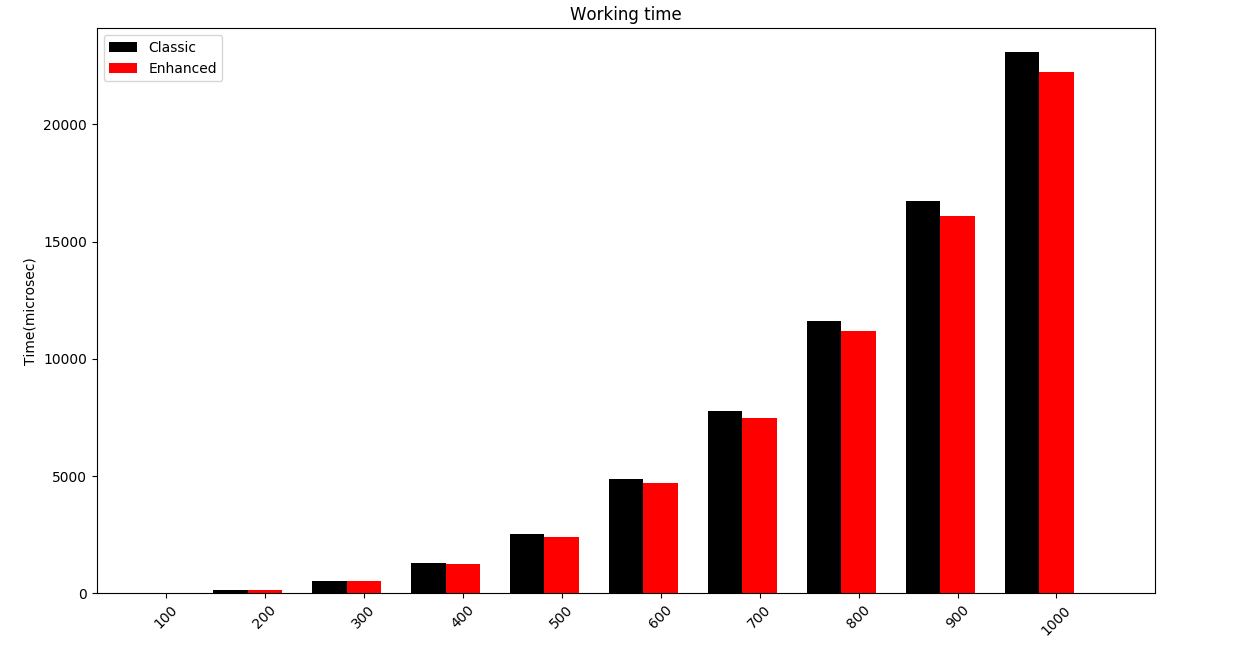
\includegraphics[width=1.1\textwidth]{img/even.png}
		\caption{График для квадратных матриц четной размерности}}
\end{figure}

\begin{figure}[ht!]
	\centering{ 
		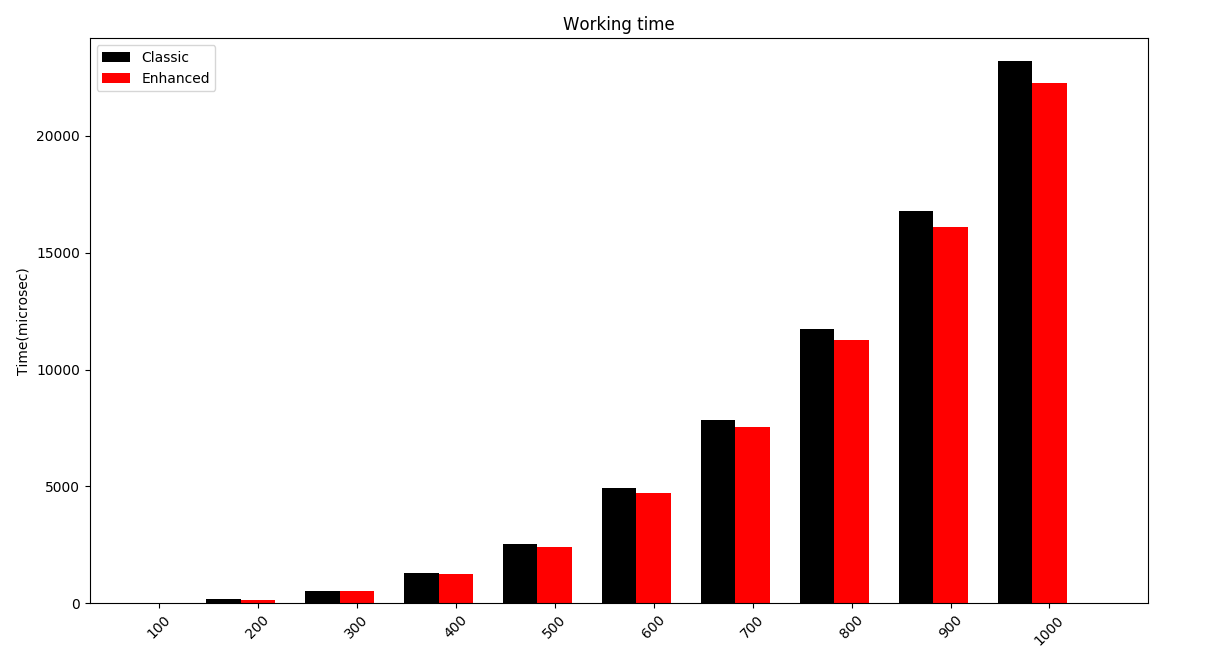
\includegraphics[width=1.1\textwidth]{img/nonEven.png}
		\caption{График для квадратных матриц нечетных размерностей}}
\end{figure}

